\FloatBarrier

\subsection{An Independent Check in the ECDFS}
\label{sec:ecdfs-check}

To test whether V12 works beyond COSMOS, we fit and evaluate the model in separate sky regions of the Extended Chandra Deep Field South (ECDFS).

We use the Euclid DR1 Deep Survey MER and PHZ classification catalogs from IRSA.\footnote{\href{https://irsa.ipac.caltech.edu/euclid-archive-documentation/data-access/\#catalogs}{IRSA Euclid DR1 catalog access}.}
We match Rubin DP2 objects to the MER catalog by sky position and retain nearest neighbors separated by less than \(0.3^{\prime\prime}\). We require a Euclid visible-band (VIS) detection, a zero detection-quality flag, and a spurious-detection probability below 0.2. We join the PHZ catalog by Euclid object ID and use \texttt{PHZ\_CLASSIFICATION} values of 1 for stars and 2 for galaxies.

We follow the same V12 procedure and estimate all coefficients from the
ECDFS calibration data. We first fit the stellar and galaxy profiles
using Rubin \(r\)-band measurements of Euclid DR1 reference stars and
galaxies.

Figure~\ref{fig:ecdfs-r-cc} compares the predicted and measured
completeness and contamination for the same set of Euclid DR1
matches with Rubin DP2 ECDFS. To draw the Euclid measured curve, we apply a threshold on the
stellar probability \(p_{\mathrm S}\) to the Rubin measurements and
count the stars and galaxies selected according to the Euclid labels.

The markers show what happens when we use \(p_{\mathrm S}>0.2\).
For \(24\leq r_{\mathrm{S\acute{e}rsic}}<24.5\), the model predicts
\(67.6\%\) completeness and \(55.9\%\) contamination. The values measured
with Euclid labels are \(66.7\%\) and \(50.6\%\). For
\(24.5\leq r_{\mathrm{S\acute{e}rsic}}<25\), the model predicts
\(45.2\%\) completeness and \(64.4\%\) contamination, compared with
\(52.4\%\) and \(72.9\%\) measured.

\begin{figure}[!hb]
  \centering
  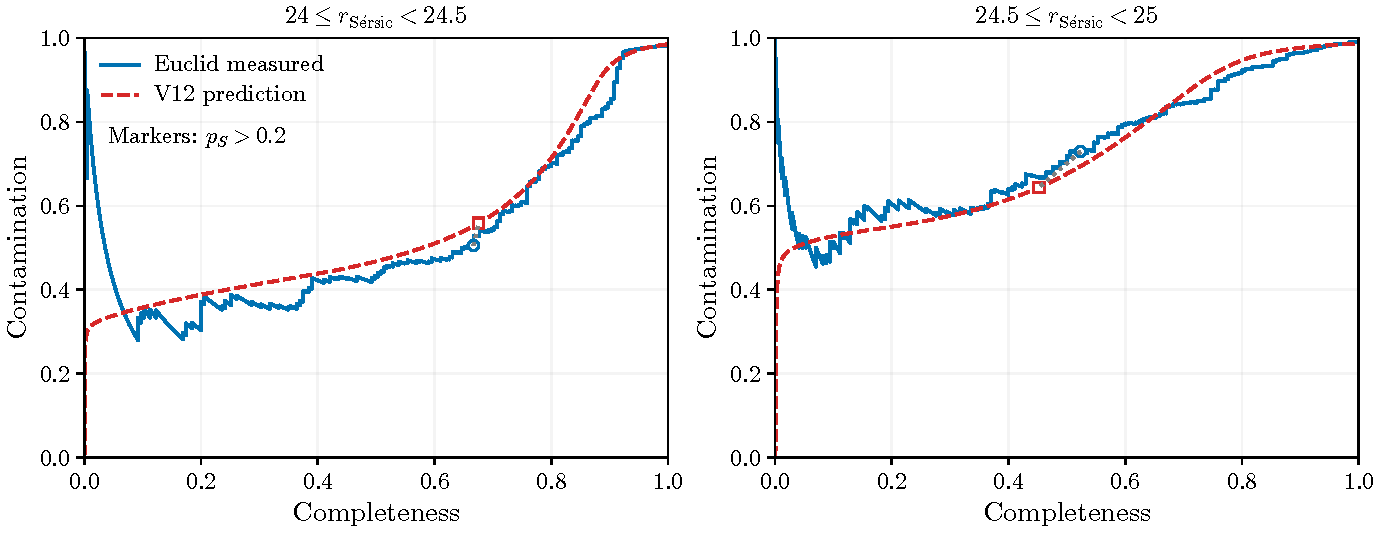
\includegraphics[width=0.85\linewidth]{ECDFS_r_performance.pdf}
  \caption{Stellar completeness and galaxy contamination in the ECDFS in
    two bins of Rubin \(r\)-band S\'{e}rsic magnitude. The solid blue
    curves are measured by counting objects with Euclid labels in the regions. The dashed red curves give the V12 predictions
    for the same sample. Open circles and squares mark the measurements
    and predictions at \(p_{\mathrm S}>0.2\), respectively.}
  \label{fig:ecdfs-r-cc}
\end{figure}
